% =====================================================================
%  skull-id-guide.tex -- Identifying Skulls
%  Build:  latexmk -pdf skull-id-guide.tex
%  Figures in skull-id-figures.tex. See README.md.
% =====================================================================
\documentclass[11pt]{article}

\usepackage[letterpaper,margin=0.8in,top=0.75in,bottom=0.8in]{geometry}
\usepackage[T1]{fontenc}
\usepackage[utf8]{inputenc}
\usepackage{lmodern}
\usepackage{microtype}
\usepackage{booktabs}
\usepackage{array}
\usepackage{tabularx}
\usepackage{xltabular}
\usepackage{multicol}
\usepackage{enumitem}
\usepackage{graphicx}
\usepackage{xcolor}
\usepackage{tikz}
\usepackage[most]{tcolorbox}
\usepackage{titlesec}
\usepackage{fancyhdr}
\usepackage[hidelinks]{hyperref}

\usetikzlibrary{calc,positioning,shapes.geometric,arrows.meta}

% Colours follow the lab handouts: dermatocranium pink, neurocranium blue,
% splanchnocranium green.
\definecolor{dermcol}{HTML}{F7D9E3}
\definecolor{neurocol}{HTML}{D3E3F2}
\definecolor{splanchcol}{HTML}{D6E8D2}
% Figure 1 codes stability, which is the axis that varies on a skull-roof map.
\definecolor{stablecol}{HTML}{D6E8D2}
\definecolor{labilecol}{HTML}{FBE3C8}
\definecolor{hingecol}{HTML}{F6D6DC}
\definecolor{bonecol}{HTML}{F2E8D5}
\definecolor{boneline}{HTML}{6B5B4A}
\definecolor{fencol}{HTML}{DCE9F2}
\definecolor{barcol}{HTML}{B5561B}
\definecolor{stubgrey}{HTML}{6E6E6E}
\definecolor{headcol}{HTML}{2E4756}

\setlist[itemize]{leftmargin=1.05em, topsep=2pt, itemsep=1.2pt, parsep=0pt}
\setlist[enumerate]{leftmargin=1.5em, topsep=2pt, itemsep=2.5pt, parsep=0pt}

\titleformat{\section}{\large\bfseries\color{headcol}}{}{0pt}{}
\titlespacing*{\section}{0pt}{13pt}{4pt}

\pagestyle{fancy}
\fancyhf{}
\lhead{\footnotesize\color{stubgrey} Identifying Skulls}
\rhead{\footnotesize\color{stubgrey} \thepage}
\renewcommand{\headrulewidth}{0.3pt}

\newcolumntype{L}[1]{>{\raggedright\arraybackslash}p{#1}}

\newtcolorbox{cladebox}[2][]{
  enhanced, breakable,
  colback=white, colframe=headcol, boxrule=0.7pt,
  arc=2pt, left=6pt, right=6pt, top=4pt, bottom=4pt,
  title={\bfseries #2}, fonttitle=\normalsize,
  coltitle=white, colbacktitle=headcol,
  attach boxed title to top left={xshift=4pt, yshift=-2pt},
  boxed title style={arc=1.5pt, boxrule=0pt}, #1
}

\newtcolorbox{watchbox}[1][]{
  enhanced, breakable,
  colback=fencol!55, colframe=barcol, boxrule=0.6pt,
  arc=2pt, left=6pt, right=6pt, top=4pt, bottom=4pt, #1
}

\newcommand{\bone}[1]{\textbf{#1}}
\newcommand{\term}[1]{\textsl{#1}}
\newcommand{\lost}{\textcolor{barcol}{\textbf{lost}}}

% =====================================================================
%  skull-id-figures.tex
%  Figures for skull-id-guide.tex. Kept separate so they can be reused
%  (and so the schematics can be exported to SVG for a web version).
%
%  Two kinds of figure live here:
%
%   * SCHEMATICS, drawn in TikZ. Always available, no licence attached,
%     ours to relabel. These are deliberately diagrams: a beginner needs
%     the topology, and an honest map teaches that better than a mediocre
%     drawing of a real skull would.
%
%   * PLATES, clipped from the literature by docs/teaching/clip-plates.py
%     into docs/teaching/plates/ (git-ignored). Every one is wrapped in
%     \IfFileExists, so the guide compiles whether or not they are there.
%     Credit lines are set by the licences and are not optional.
%
%  Requires the colours defined in skull-id-guide.tex.
% =====================================================================

% ---------------------------------------------------------------------
%  Plate helper: include if clipped, otherwise leave a visible stub
% ---------------------------------------------------------------------
\newcommand{\plate}[4]{%
  % #1 = file stem in plates/  #2 = width  #3 = caption  #4 = credit
  \par\medskip
  \IfFileExists{plates/#1.png}{%
    \begin{center}\includegraphics[width=#2\linewidth]{plates/#1}\end{center}
    \vspace{-2pt}
    {\footnotesize #3\ {\color{stubgrey}\itshape #4}\par}
  }{%
    \begin{center}
      \fcolorbox{stubgrey}{white}{\parbox{0.86\linewidth}{\footnotesize
        \color{stubgrey}\textbf{Plate not clipped:} \texttt{plates/#1.png}.
        Run \texttt{python3 docs/teaching/clip-plates.py} with the PDFs in
        \texttt{papers/}.\\[3pt] #3\ \itshape #4}}
    \end{center}
  }%
  \par\medskip
}

% =====================================================================
%  FIGURE 1: skull-roof topology map
%  Tiles in their correct relative positions. What a beginner has to hold
%  is which bone touches which, so this is drawn as a map. Coordinates are
%  in centimetres so nothing collides when the text width changes.
% =====================================================================
\tikzset{
  bonetile/.style  = {draw=boneline, line width=0.5pt, rounded corners=1.5pt,
                      font=\scriptsize, align=center, inner sep=2.2pt,
                      minimum height=0.48cm},
  tstable/.style   = {bonetile, fill=stablecol},   % present, in position, ~always
  tlabile/.style   = {bonetile, fill=labilecol},   % lost or fused somewhere
  thinge/.style    = {bonetile, fill=hingecol},    % leaves the jaw in mammals
}

% \bonetile places a bone box at a named coordinate, rotated to sit roughly
% the way the bone sits. Contact lines are drawn BEFORE the boxes, so each one
% is occluded except where it crosses the gap between two neighbours -- which
% is exactly where an articulation is.
\tikzset{
  bonebox/.style   = {draw=boneline, line width=0.5pt, rounded corners=1.2pt,
                      align=center, inner xsep=1.6pt, inner ysep=1pt,
                      font=\tiny},
  bstable/.style   = {bonebox, fill=stablecol},
  blabile/.style   = {bonebox, fill=labilecol},
  bhinge/.style    = {bonebox, fill=hingecol},
  bdeep/.style     = {bonebox, fill=hingecol, densely dashed},
  bextra/.style    = {bonebox, fill=stubgrey!22},
  contact/.style   = {draw=stubgrey, line width=0.4pt},
  leader/.style    = {draw=stubgrey, line width=0.4pt},
  exlab/.style     = {font=\scriptsize, color=black, inner sep=1pt, align=left},
}

\newcommand{\figBoneMap}{%
  \par\medskip
  \noindent\begin{minipage}{\linewidth}
  \centering
  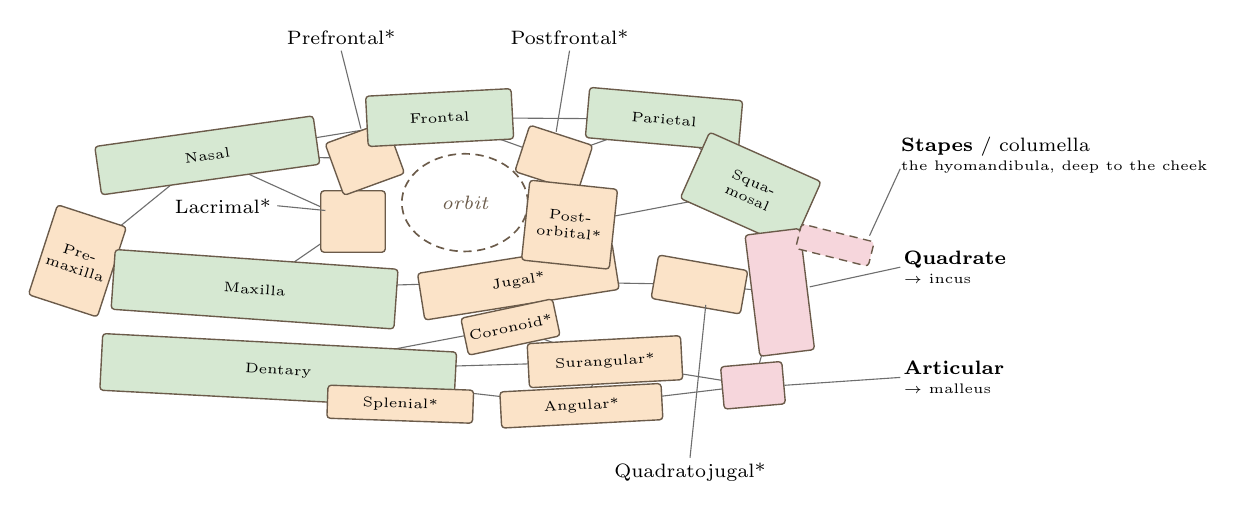
\begin{tikzpicture}[x=1cm, y=1cm]

    % ---------- bone centres -------------------------------------------
    \coordinate (pmx) at (0.80,2.28);   \coordinate (mx)  at (3.05,1.92);
    \coordinate (na)  at (2.45,3.62);   \coordinate (la)  at (4.30,2.78);
    \coordinate (prf) at (4.45,3.58);   \coordinate (fr)  at (5.40,4.10);
    \coordinate (pof) at (6.85,3.58);   \coordinate (po)  at (7.05,2.74);
    \coordinate (pa)  at (8.25,4.08);   \coordinate (ju)  at (6.40,2.02);
    \coordinate (sq)  at (9.35,3.18);   \coordinate (qj)  at (8.70,1.98);
    \coordinate (qu)  at (9.72,1.88);   \coordinate (st)  at (10.42,2.48);
    \coordinate (de)  at (3.35,0.88);   \coordinate (co)  at (6.30,1.44);
    \coordinate (sa)  at (7.50,1.00);   \coordinate (an)  at (7.20,0.44);
    \coordinate (sp)  at (4.90,0.46);   \coordinate (ar)  at (9.38,0.70);

    % ---------- articulations (drawn first, occluded by the boxes) ------
    \foreach \bxa/\bxb in {pmx/mx, pmx/na, na/fr, na/prf, na/la, mx/la, mx/ju,
                           la/prf, prf/fr, fr/pof, fr/pa, pof/po, pof/pa,
                           po/ju, po/sq, pa/sq, ju/qj, qj/qu, sq/qu, qu/ar,
                           de/sp, de/co, de/sa, de/an, sa/an, sa/ar, an/ar,
                           co/sa, sq/st}
      {\draw[contact] (\bxa) -- (\bxb);}

    % ---------- orbit ---------------------------------------------------
    \draw[draw=boneline, line width=0.6pt, densely dashed]
      (5.72,3.02) ellipse (0.80 and 0.62);
    \node[font=\scriptsize\itshape, color=boneline] at (5.72,3.02) {orbit};

    % ---------- upper skull --------------------------------------------
    \node[blabile, minimum width=0.92cm, minimum height=1.20cm, rotate=-18] at (pmx)
      {Pre-\\maxilla};
    \node[bstable, minimum width=3.6cm, minimum height=0.76cm, rotate=-4] at (mx) {Maxilla};
    \node[bstable, minimum width=2.8cm, minimum height=0.62cm, rotate=8]  at (na) {Nasal};
    \node[blabile, minimum width=0.82cm, minimum height=0.78cm] at (la) {};
    \node[blabile, minimum width=0.82cm, minimum height=0.70cm, rotate=20] at (prf) {};
    \node[bstable, minimum width=1.85cm, minimum height=0.64cm, rotate=3]  at (fr) {Frontal};
    \node[blabile, minimum width=0.84cm, minimum height=0.62cm, rotate=-18] at (pof) {};
    \node[blabile, minimum width=2.5cm, minimum height=0.60cm, rotate=9]  at (ju) {Jugal*};
    \node[blabile, minimum width=1.12cm, minimum height=1.02cm, rotate=-6] at (po)
      {Post-\\orbital*};
    \node[bstable, minimum width=1.95cm, minimum height=0.64cm, rotate=-5] at (pa) {Parietal};
    \node[bstable, minimum width=1.55cm, minimum height=0.92cm, rotate=-24] at (sq)
      {Squa-\\mosal};
    \node[blabile, minimum width=1.15cm, minimum height=0.56cm, rotate=-10] at (qj) {};
    \node[bhinge, minimum width=0.70cm, minimum height=1.55cm, rotate=7] at (qu) {};
    

    % ---------- lower jaw ------------------------------------------------
    \node[bstable, minimum width=4.5cm, minimum height=0.72cm, rotate=-3] at (de) {Dentary};
    \node[blabile, minimum width=0.98cm, minimum height=0.48cm, rotate=12] at (co)
      {Coronoid*};
    \node[blabile, minimum width=1.95cm, minimum height=0.56cm, rotate=3] at (sa)
      {Surangular*};
    \node[blabile, minimum width=2.05cm, minimum height=0.46cm, rotate=3] at (an)
      {Angular*};
    \node[blabile, minimum width=1.85cm, minimum height=0.42cm, rotate=-2] at (sp)
      {Splenial*};
    \node[bhinge, minimum width=0.78cm, minimum height=0.54cm, rotate=5] at (ar) {};
    \node[bdeep,  minimum width=0.95cm, minimum height=0.32cm, rotate=-14] at (st) {};

    % ---------- external labels: the small, crowded elements -------------
    % above the roof
    \draw[leader] (4.40,3.96) -- (4.15,4.95);
    \node[exlab, anchor=south] at (4.15,4.98) {Prefrontal*};
    \draw[leader] (6.88,3.92) -- (7.05,4.95);
    \node[exlab, anchor=south] at (7.05,4.98) {Postfrontal*};
    % in front
    \draw[leader] (3.95,2.92) -- (3.34,2.98);
    \node[exlab, anchor=east] at (3.30,2.98) {Lacrimal*};
    % behind
    \draw[leader] (10.86,2.60) -- (11.25,3.45);
    \node[exlab, anchor=west] at (11.22,3.62)
      {\textbf{Stapes} / columella\\[-1pt]{\tiny the hyomandibula, deep to the cheek}};
    \draw[leader] (10.10,1.95) -- (11.25,2.20);
    \node[exlab, anchor=west] at (11.25,2.20)
      {\textbf{Quadrate}\\[-1pt]{\tiny$\rightarrow$ incus}};
    \draw[leader] (9.78,0.70) -- (11.25,0.80);
    \node[exlab, anchor=west] at (11.25,0.80)
      {\textbf{Articular}\\[-1pt]{\tiny$\rightarrow$ malleus}};
    \draw[leader] (8.78,1.72) -- (8.58,-0.22);
    \node[exlab, anchor=north] at (8.58,-0.25) {Quadratojugal*};
    

    % ---------- the jaw joint -------------------------------------------
    

  \end{tikzpicture}

  \vspace{2pt}
  {\footnotesize\raggedright Generalised amniote, left lateral view. Boxes sit
   roughly where and how the bones sit, and the thin grey lines mark the usual
   contacts. The two pink elements meet at the jaw joint, and the stapes is
   dashed because it lies deep to the cheek.\par}
  \vspace{4pt}
  {\footnotesize\raggedright
   \tikz[baseline=-0.6ex]\node[bstable, minimum width=0.42cm,
     minimum height=0.28cm]{};\,\textbf{Stable}: present, and in this position,
   across essentially all bony jawed vertebrates.\quad
   \tikz[baseline=-0.6ex]\node[blabile, minimum width=0.42cm,
     minimum height=0.28cm]{};\,\textbf{Labile*}: lost or fused to a neighbour
   somewhere, and worth learning as absences.\quad
   \tikz[baseline=-0.6ex]\node[bhinge, minimum width=0.42cm,
     minimum height=0.28cm]{};\,\textbf{Hinge}: leaves the jaw entirely in
   mammals.\par}
  \end{minipage}
  \par\medskip
}

% =====================================================================
%  FIGURES 0a/0b: where the bones come from
%  Derivation trees for the neurocranium and the first two arches. Deliberately
%  uncoloured: figure 1 already spends colour on stability, and reusing the
%  lab's unit colours here would make pink and green mean two things each.
% =====================================================================
\tikzset{
  srcbox/.style  = {draw=boneline, line width=0.7pt, rounded corners=2pt,
                    fill=bonecol!70, font=\scriptsize\bfseries, align=center,
                    inner sep=3pt, minimum height=0.6cm},
  derbox/.style  = {draw=boneline, line width=0.4pt, rounded corners=2pt,
                    fill=bonecol!35, font=\tiny, align=center,
                    inner sep=2.5pt, minimum height=0.55cm},
  endbox/.style  = {derbox, fill=white, densely dashed},
  flow/.style    = {-{Stealth[length=4pt]}, draw=barcol, line width=0.6pt},
  qual/.style    = {font=\tiny\itshape, color=stubgrey, align=left},
}

\newcommand{\figNeurocranium}{%
  \par\smallskip
  \noindent\begin{minipage}{\linewidth}
  \centering
  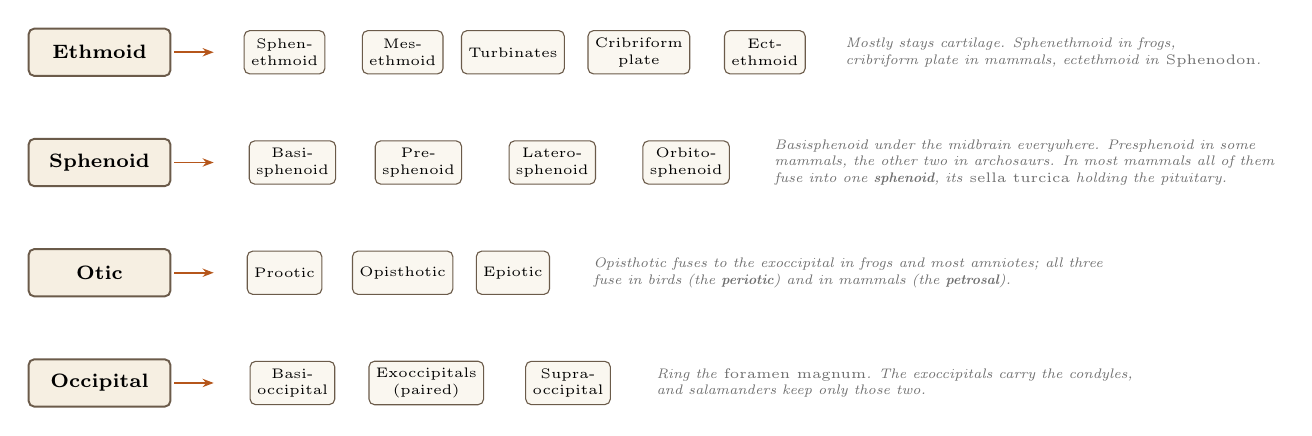
\begin{tikzpicture}[x=1cm, y=1cm]
    \foreach \yy/\name in {4.35/Ethmoid, 2.95/Sphenoid, 1.55/Otic, 0.15/Occipital}
      {\node[srcbox, minimum width=1.8cm] at (0.9,\yy) {\name};
       \draw[flow] (1.85,\yy) -- (2.35,\yy);}

    % ethmoid
    \node[derbox] (e1) at (3.25,4.35) {Sphen-\\ethmoid};
    \node[derbox] (e2) at (4.75,4.35) {Mes-\\ethmoid};
    \node[derbox] (e3) at (6.15,4.35) {Turbinates};
    \node[derbox] (e4) at (7.75,4.35) {Cribriform\\plate};
    \node[derbox] (e5) at (9.35,4.35) {Ect-\\ethmoid};
    \node[qual, anchor=west] at (10.25,4.35)
      {Mostly stays cartilage. Sphenethmoid in frogs,\\
       cribriform plate in mammals, ectethmoid in \emph{Sphenodon}.};

    % sphenoid
    \node[derbox] (s1) at (3.35,2.95) {Basi-\\sphenoid};
    \node[derbox] (s2) at (4.95,2.95) {Pre-\\sphenoid};
    \node[derbox] (s3) at (6.65,2.95) {Latero-\\sphenoid};
    \node[derbox] (s4) at (8.35,2.95) {Orbito-\\sphenoid};
    \node[qual, anchor=west] at (9.35,2.95)
      {Basisphenoid under the midbrain everywhere. Presphenoid in some\\
       mammals, the other two in archosaurs. In most mammals all of them\\
       fuse into one \textbf{sphenoid}, its \emph{sella turcica} holding the pituitary.};

    % otic
    \node[derbox] (o1) at (3.25,1.55) {Prootic};
    \node[derbox] (o2) at (4.75,1.55) {Opisthotic};
    \node[derbox] (o3) at (6.15,1.55) {Epiotic};
    \node[qual, anchor=west] at (7.05,1.55)
      {Opisthotic fuses to the exoccipital in frogs and most amniotes; all three\\
       fuse in birds (the \textbf{periotic}) and in mammals (the \textbf{petrosal}).};

    % occipital
    \node[derbox] (c1) at (3.35,0.15) {Basi-\\occipital};
    \node[derbox] (c2) at (5.05,0.15) {Exoccipitals\\(paired)};
    \node[derbox] (c3) at (6.85,0.15) {Supra-\\occipital};
    \node[qual, anchor=west] at (7.85,0.15)
      {Ring the \emph{foramen magnum}. The exoccipitals carry the condyles,\\
       and salamanders keep only those two.};
  \end{tikzpicture}

  \vspace{2pt}
  {\footnotesize\raggedright The four neurocranial ossification centers (anterior to posterior) \& their derivatives.\par}
  \end{minipage}
  \par\smallskip
}

\newcommand{\figArches}{%
  \par\smallskip
  \noindent\begin{minipage}{\linewidth}
  \centering
  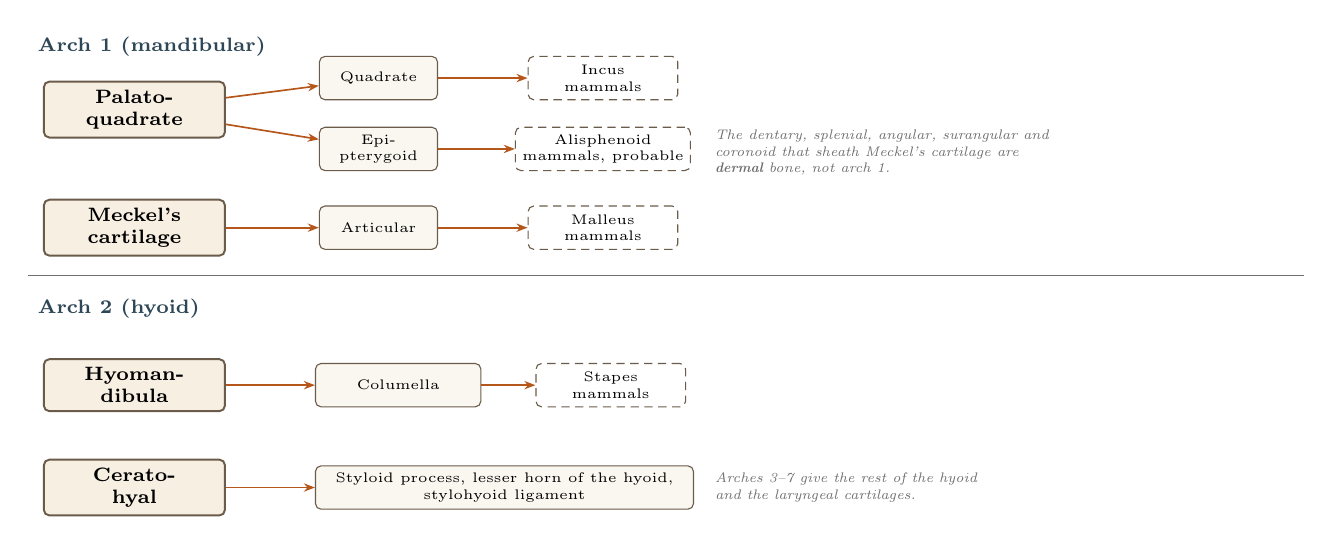
\begin{tikzpicture}[x=1cm, y=1cm]
    % ---------------- arch 1
    \node[font=\scriptsize\bfseries, color=headcol, anchor=west] at (0,3.75)
      {Arch 1 (mandibular)};
    \node[srcbox, minimum width=2.3cm] (pq) at (1.35,2.95) {Palato-\\quadrate};
    \node[srcbox, minimum width=2.3cm] (mc) at (1.35,1.45) {Meckel's\\cartilage};

    \node[derbox, minimum width=1.5cm] (qd) at (4.45,3.35) {Quadrate};
    \node[derbox, minimum width=1.5cm] (ep) at (4.45,2.45) {Epi-\\pterygoid};
    \node[derbox, minimum width=1.5cm] (ar) at (4.45,1.45) {Articular};

    \node[endbox, minimum width=1.9cm] (ic) at (7.30,3.35) {Incus\\{\tiny mammals}};
    \node[endbox, minimum width=1.9cm] (al) at (7.30,2.45) {Alisphenoid\\{\tiny mammals, probable}};
    \node[endbox, minimum width=1.9cm] (ma) at (7.30,1.45) {Malleus\\{\tiny mammals}};

    \foreach \a/\b in {pq/qd, pq/ep, mc/ar} {\draw[flow] (\a) -- (\b);}
    \foreach \a/\b in {qd/ic, ep/al, ar/ma} {\draw[flow] (\a) -- (\b);}

    \node[qual, anchor=west] at (8.60,2.40)
      {The dentary, splenial, angular, surangular and\\
       coronoid that sheath Meckel's cartilage are\\
       \textbf{dermal} bone, not arch 1.};

    % ---------------- arch 2
    \draw[draw=stubgrey, line width=0.3pt] (0,0.85) -- (16.2,0.85);
    \node[font=\scriptsize\bfseries, color=headcol, anchor=west] at (0,0.42)
      {Arch 2 (hyoid)};
    \node[srcbox, minimum width=2.3cm] (hm) at (1.35,-0.55) {Hyoman-\\dibula};
    \node[srcbox, minimum width=2.3cm] (ch) at (1.35,-1.85) {Cerato-\\hyal};

    \node[derbox, minimum width=2.1cm] (cl) at (4.70,-0.55) {Columella};
    \node[endbox, minimum width=1.9cm] (st) at (7.40,-0.55) {Stapes\\{\tiny mammals}};
    \node[derbox, minimum width=4.8cm] (sty) at (6.05,-1.85)
      {Styloid process, lesser horn of the hyoid,\\stylohyoid ligament};

    \foreach \a/\b in {hm/cl, cl/st, ch/sty} {\draw[flow] (\a) -- (\b);}
    \node[qual, anchor=west] at (8.60,-1.85)
      {Arches 3--7 give the rest of the hyoid\\and the laryngeal cartilages.};
  \end{tikzpicture}

  \vspace{2pt}
  {\footnotesize\raggedright The first two pharyngeal arches.\par}
  \end{minipage}
  \par\smallskip
}

% =====================================================================
%  FIGURE 1b: the same stylised skull across four groups
%  Same coordinates as figure 1, carrying the bone abbreviations. A bone that
%  a group lacks is simply not drawn, so the silhouette of what is missing is
%  the whole point. Codes are baked into the \bXX macros so the panels and the
%  caption key cannot drift apart.
% =====================================================================
% #1 x  #2 y  #3 w  #4 h  #5 rotation  #6 style  #7 abbreviation
\newcommand{\bn}[7]{\node[#6, minimum width=#3cm, minimum height=#4cm,
  rotate=#5, inner xsep=1pt, inner ysep=0.5pt] at (#1,#2) {#7};}

% every element of the generalised skull, as its own macro
\newcommand{\bPMX}[1]{\bn{0.80}{2.28}{0.92}{1.20}{-18}{#1}{PM}}
\newcommand{\bMX} [1]{\bn{3.05}{1.92}{3.60}{0.76}{-4}{#1}{MX}}
\newcommand{\bNA} [1]{\bn{2.45}{3.62}{2.80}{0.62}{8}{#1}{NA}}
\newcommand{\bLA} [1]{\bn{4.30}{2.78}{0.82}{0.78}{0}{#1}{LA}}
\newcommand{\bPRF}[1]{\bn{4.45}{3.58}{0.82}{0.70}{20}{#1}{PRF}}
\newcommand{\bFR} [1]{\bn{5.40}{4.10}{1.85}{0.64}{3}{#1}{FR}}
\newcommand{\bPOF}[1]{\bn{6.85}{3.58}{0.84}{0.62}{-18}{#1}{POF}}
\newcommand{\bPO} [1]{\bn{7.05}{2.74}{1.12}{1.02}{-6}{#1}{PO}}
\newcommand{\bPA} [1]{\bn{8.25}{4.08}{1.95}{0.64}{-5}{#1}{PA}}
\newcommand{\bJU} [1]{\bn{6.40}{2.02}{2.50}{0.60}{9}{#1}{JU}}
\newcommand{\bSQ} [1]{\bn{9.35}{3.18}{1.55}{0.92}{-24}{#1}{SQ}}
\newcommand{\bQJ} [1]{\bn{8.70}{1.98}{1.15}{0.56}{-10}{#1}{QJ}}
\newcommand{\bQU} [1]{\bn{9.72}{1.88}{0.70}{1.55}{7}{#1}{QU}}
\newcommand{\bST} [1]{\bn{10.98}{2.62}{0.95}{0.32}{-14}{#1}{ST}}
\newcommand{\bDE} [1]{\bn{3.35}{0.88}{4.50}{0.72}{-3}{#1}{DE}}
\newcommand{\bCO} [1]{\bn{6.30}{1.44}{0.98}{0.48}{12}{#1}{CO}}
\newcommand{\bSA} [1]{\bn{7.50}{1.00}{1.95}{0.56}{3}{#1}{SA}}
\newcommand{\bAN} [1]{\bn{7.20}{0.44}{2.05}{0.46}{3}{#1}{AN}}
\newcommand{\bSP} [1]{\bn{4.90}{0.46}{1.85}{0.42}{-2}{#1}{SP}}
\newcommand{\bAR} [1]{\bn{9.38}{0.70}{0.78}{0.54}{5}{#1}{AR}}
\newcommand{\bORB}{\draw[draw=boneline, line width=0.5pt, densely dashed]
  (5.72,3.02) ellipse (0.80 and 0.62);}

% \minipanel{caption}{body}
\newcommand{\minipanel}[2]{%
  \begin{minipage}[t]{0.48\linewidth}
    \centering
    \begin{tikzpicture}[scale=0.55, transform shape, x=1cm, y=1cm,
        every node/.append style={font=\large\bfseries}]
      #2
    \end{tikzpicture}\\[1pt]
    {\raggedright\scriptsize #1\par}
  \end{minipage}%
}

\newcommand{\figSkullVariants}{%
  \par\medskip
  \noindent
  \minipanel{\textbf{Actinopterygian.} Generalized skull retains everything with some bonus bones. Many, \textit{many} actinopterygians reduce and alter their skull dramatically. The base, ``generic'' skull has well over a hundred elements.}{%
      \bORB \bPMX{bstable}\bMX{bstable}\bNA{bstable}\bLA{blabile}\bPRF{blabile}
      \bFR{bstable}\bPOF{blabile}\bJU{blabile}\bPO{blabile}\bPA{bstable}
      \bSQ{bstable}\bQJ{blabile}\bQU{bhinge}\bDE{bstable}\bCO{blabile}
      \bSA{blabile}\bAN{blabile}\bSP{blabile}\bAR{bhinge}
      \bn{10.95}{2.20}{1.20}{2.00}{-5}{bextra}{POP}
      \bn{12.35}{3.00}{1.50}{2.20}{-6}{bextra}{OP}
      \bn{12.45}{1.35}{1.30}{1.20}{-8}{bextra}{SOP}
      \bn{11.30}{0.35}{2.20}{0.50}{-12}{bextra}{BR}}
  \hfill
  \minipanel{\textbf{Salamander.} Jugal, quadratojugal, postorbital, postfrontal
    and lacrimal all lost.}{%
      \bORB \bPMX{bstable}\bMX{bstable}\bNA{bstable}\bPRF{blabile}
      \bFR{bstable}\bPA{bstable}\bSQ{bstable}\bQU{bhinge}\bST{bdeep}
      \bDE{bstable}\bCO{blabile}\bSA{blabile}\bAN{blabile}\bSP{blabile}
      \bAR{bhinge}}
  \par\medskip
  \noindent
  \minipanel{\textbf{Lizard.} The quadratojugal is lost, resulting in no lower temporal bar and a situation where the quadrate can swing freely on the squamosal.}{%
      \bORB \bPMX{bstable}\bMX{bstable}\bNA{bstable}\bLA{blabile}\bPRF{blabile}
      \bFR{bstable}\bPOF{blabile}\bJU{blabile}\bPO{blabile}\bPA{bstable}
      \bSQ{bstable}\bQU{bhinge}\bST{bdeep}\bDE{bstable}\bCO{blabile}
      \bSA{blabile}\bAN{blabile}\bSP{blabile}\bAR{bhinge}}
  \hfill
  \minipanel{\textbf{Mammal.} Lower jaw is only the mandible, with the post-dentary bones moving or fusing. The jaw joint is now dentary to squamosal directly. Postorbital, postfrontal, prefrontal and quadratojugal all lost.}{%
      \bORB \bPMX{bstable}\bMX{bstable}\bNA{bstable}\bLA{blabile}
      \bFR{bstable}\bJU{blabile}\bPA{bstable}\bSQ{bstable}
      \bDE{bstable}
      \bn{10.80}{3.20}{0.80}{0.55}{8}{bhinge}{IN}
      \bn{12.00}{3.20}{0.85}{0.55}{-4}{bhinge}{MA}
      \bn{13.20}{3.20}{0.80}{0.45}{-10}{bdeep}{ST}}
  \par\medskip
  {\footnotesize\raggedright Generalized skull diagrams for major clades. Colors as in the map above; grey boxes show bones actinopterygians have that aren't part of the tetrapod skull.
   AN, angular; AR, articular; BR, branchiostegals; CO, coronoid; DE, dentary;
   FR, frontal; IN, incus; JU, jugal; LA, lacrimal; MA, malleus; MX, maxilla;
   NA, nasal; OP, opercular; PA, parietal; PM, premaxilla; PO, postorbital;
   POF, postfrontal; POP, preopercular; PRF, prefrontal; QJ, quadratojugal; QU, quadrate; SA,
   surangular; SOP, subopercular; SP, splenial; SQ, squamosal; ST, stapes.\par}
  \par\medskip
}

% =====================================================================
%  FIGURE 2: the temporal series
% =====================================================================
\tikzset{
  skullfill/.style = {fill=bonecol, draw=boneline, line width=0.6pt},
  openfill/.style  = {fill=white, draw=boneline, line width=0.5pt},
  fenfill/.style   = {fill=fencol, draw=boneline, line width=0.5pt},
  barbold/.style   = {draw=barcol, line width=1.7pt, line cap=round},
  cuthint/.style   = {draw=barcol, line width=0.8pt,
                      dash pattern=on 2pt off 1.7pt},
}

% Generic amniote lateral silhouette. Snout left, occiput right.
\newcommand{\skulloutline}{%
  \path[skullfill]
    (0,0.60)
      .. controls (0.55,1.00) and (1.35,1.22) .. (2.15,1.26)
      .. controls (2.85,1.29) and (3.32,1.16) .. (3.42,0.90)
    -- (3.38,0.34) -- (2.60,0.16) -- (0.06,0.14) -- cycle;
}
% Orbit and naris never move. That is the point: only the back changes.
\newcommand{\skullorbit}{%
  \path[openfill] (1.85,0.76) circle (0.30);
  \path[openfill] (0.30,0.66) ellipse (0.12 and 0.09);
}

% \fenpanel{title}{note}{extra tikz}
\newcommand{\fenpanel}[3]{%
  \begin{minipage}[t]{0.235\linewidth}
    \centering
    \begin{tikzpicture}[scale=1.02]
      \skulloutline #3 \skullorbit
    \end{tikzpicture}\\[3pt]
    {\footnotesize\bfseries #1}\\[2pt]
    \begin{minipage}{\linewidth}
      \raggedright\scriptsize\color{stubgrey}\setlength{\parskip}{0pt}#2
    \end{minipage}
  \end{minipage}%
}

\newcommand{\figFenestration}{%
  \par\medskip
  \noindent
  \begin{tabular}{@{}c@{\hspace{0.012\linewidth}}c@{\hspace{0.012\linewidth}}%
                   c@{\hspace{0.012\linewidth}}c@{}}
  \fenpanel{Anapsid}{No opening at all. Stem amniotes, and the starting
    condition for everything else in this figure.}{}
  &
  \fenpanel{Synapsid}{One opening, and it is \emph{low}. The postorbital
    and squamosal meet above it to close the top.}{%
      \path[fenfill] (2.72,0.55) ellipse (0.33 and 0.20);
      \draw[barbold] (2.32,0.92) -- (3.20,0.88);}
  &
  \fenpanel{Diapsid}{Two openings, one above the other, separated by the
    postorbital--squamosal bar. Tuatara, crocodilians.}{%
      \path[fenfill] (2.78,1.02) ellipse (0.32 and 0.14);
      \path[fenfill] (2.74,0.55) ellipse (0.31 and 0.19);
      \draw[barbold] (2.34,0.82) -- (3.22,0.78);
      \draw[barbold] (2.36,0.28) -- (3.30,0.30);}
  &
  \fenpanel{Lizard}{Upper opening and its bar kept. The \emph{lower bar}
    is gone, so that opening runs out to the margin.}{%
      \path[fenfill] (2.78,1.02) ellipse (0.32 and 0.14);
      \path[fenfill] (2.28,0.62) -- (3.36,0.58) -- (3.38,0.22)
                     -- (2.52,0.16) -- cycle;
      \draw[barbold] (2.34,0.82) -- (3.22,0.78);
      \draw[cuthint] (2.42,0.24) -- (3.34,0.26);}
  \\[10pt]
  \fenpanel{Turtle}{No fenestra anywhere, but the cheek is deeply
    \emph{emarginated}, notched inwards from the free rear edge.}{%
      \path[fill=white]
        (3.46,1.02) .. controls (2.88,0.86) and (2.74,0.46) ..
        (3.04,0.12) -- (3.54,0.12) -- (3.54,1.02) -- cycle;
      \draw[draw=boneline, line width=0.6pt]
        (3.42,0.92) .. controls (2.88,0.84) and (2.76,0.46) ..
        (3.05,0.14);}
  &
  \fenpanel{Bird}{Postorbital bar lost, so orbit and temporal region run
    together into one great opening. The jugal bar is a bare rod.}{%
      \path[fill=white, draw=boneline, line width=0.5pt]
        (2.12,1.10) .. controls (2.70,1.12) and (3.06,0.96) ..
        (3.14,0.64) .. controls (3.00,0.48) and (2.50,0.50) ..
        (2.14,0.56) -- cycle;
      \draw[barbold] (1.30,0.28) -- (3.20,0.33);}
  &
  \fenpanel{Mammal}{One opening, hugely enlarged; postorbital bar usually
    gone, and the \emph{zygomatic arch} forms the floor of the fossa.}{%
      \path[fill=white, draw=boneline, line width=0.5pt]
        (2.08,1.16) .. controls (2.80,1.18) and (3.24,1.00) ..
        (3.30,0.62) .. controls (3.00,0.50) and (2.40,0.52) ..
        (2.10,0.58) -- cycle;
      \draw[barbold] (1.55,0.42) .. controls (2.40,0.28) and (3.00,0.30)
        .. (3.32,0.42);}
  &
  \begin{minipage}[t]{0.235\linewidth}
    \raggedright\footnotesize
    \textbf{Reading the panels}\\[3pt]
    {\scriptsize
     \tikz[baseline=-0.5ex]\draw[barbold](0,0)--(0.5,0); \; a \textbf{bar}:
     bone you can trace with a finger.\\[3pt]
     \tikz[baseline=-0.5ex]\path[fenfill](0,0) ellipse (0.26 and 0.13);
     \; a \textbf{fenestra}: a hole ringed by bone.\\[3pt]
     \tikz[baseline=-0.5ex]\draw[cuthint](0,0)--(0.5,0); \; where a bar has
     been \textbf{lost}.\\[4pt]
     Orbit and nostril are drawn in the same place every time. Only the
     temporal region changes.}
  \end{minipage}
  \end{tabular}
  \par\medskip
}

% =====================================================================
%  FIGURE 3: the jaw joint becomes the middle ear
% =====================================================================
\newcommand{\figOssicles}{%
  \par\medskip
  \begin{center}
  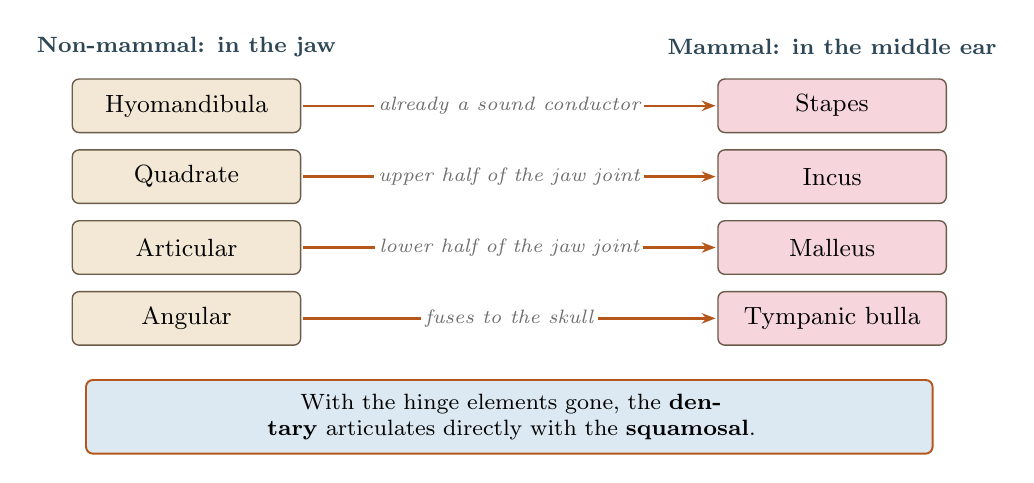
\begin{tikzpicture}[x=1cm, y=1cm,
      oldbox/.style={draw=boneline, line width=0.5pt, rounded corners=2.5pt,
                     fill=bonecol, font=\small, align=center,
                     minimum width=2.9cm, minimum height=0.68cm},
      newbox/.style={draw=boneline, line width=0.5pt, rounded corners=2.5pt,
                     fill=hingecol, font=\small, align=center,
                     minimum width=2.9cm, minimum height=0.68cm},
      arr/.style={-{Stealth[length=5pt]}, line width=0.9pt, color=barcol},
      viaz/.style={font=\scriptsize\itshape, color=stubgrey, align=center,
                   fill=white, inner sep=1.5pt}]

    \node[font=\footnotesize\bfseries, color=headcol] at (0,3.45)
      {Non-mammal: in the jaw};
    \node[font=\footnotesize\bfseries, color=headcol] at (8.2,3.45)
      {Mammal: in the middle ear};

    \foreach \y/\old/\new/\via in {
        2.7/Hyomandibula/Stapes/{already a sound conductor},
        1.8/Quadrate/Incus/{upper half of the jaw joint},
        0.9/Articular/Malleus/{lower half of the jaw joint},
        0.0/Angular/{Tympanic bulla}/{fuses to the skull}}
    {
      \node[oldbox] (o) at (0,\y) {\old};
      \node[newbox] (n) at (8.2,\y) {\new};
      \draw[arr] (1.48,\y) -- (6.72,\y);
      \node[viaz] at (4.1,\y) {\via};
    }

    \node[draw=barcol, line width=0.7pt, rounded corners=2.5pt,
          fill=fencol, font=\footnotesize, align=center, text width=10.4cm,
          inner sep=5pt]
      at (4.1,-1.25)
      {With the hinge elements gone, the \textbf{dentary} articulates directly with the \textbf{squamosal}.};
  \end{tikzpicture}
  \end{center}
  \par\medskip
}


% ======================================================================
\begin{document}

\begin{center}
  {\LARGE\bfseries\color{headcol} Identifying Skulls}
\end{center}
\vspace{2pt}
\hrule height 0.8pt
\vspace{6pt}

% ======================================================================
\section{Three Skull ``Zones''}

\begin{itemize}
\item \bone{Neurocranium} (brain case): endochondral bone replacing the
  cartilage capsule around brain, ear and nose. Four ossification centers: \term{ethmoid}, \term{sphenoid}, \term{otic}, \term{occipital}.
\item \bone{Splanchnocranium} (pharyngeal arches): Arch 1 gives the
  \bone{palatoquadrate} and \bone{Meckel's cartilage}, arch 2 the
  \bone{hyomandibula}, arches 3--7 the gill skeleton (hyoid and
  larynx in tetrapods).
\item \bone{Dermatocranium} (everything else): Dermal bone that ossifies in the skin without a cartilage precursor. The dermatocranium is the most labile, and frequently loses bones. In series:
  \emph{midline} (nasal, frontal, parietal, postparietal), \emph{marginal
  tooth-bearing} (premaxilla, maxilla, septomaxilla), \emph{circumorbital}
  (lacrimal, prefrontal, postfrontal, postorbital, jugal), \emph{cheek}
  (squamosal, quadratojugal), \emph{opercular} (preopercular, opercular,
  subopercular, branchiostegals; lost in tetrapods), \emph{palate} (vomer,
  pterygoid, palatine, ectopterygoid), and the sheath around Meckel's cartilage
  (dentary, splenial, angular, surangular, coronoid, prearticular).
\end{itemize}

Different bones in the skull often end up fusing to each other, producing composite bones (e.g., frontoparietal). Mammals and birds have high degrees of bone fusion, but if you examine the \textit{Amia} skull you can see a highly unfused state.

\subsection*{Neurocranium derivatives}
\figNeurocranium

\subsection*{Splanchnocranium derivatives}
\figArches

\section{General skull map}

\figBoneMap

\figSkullVariants


\section{The jaw joint and the ear}

\figOssicles

\noindent
{\footnotesize Vertebrates have lower jaws in many separate bones (often five or more), with the jaw joint being between the quadrate and the articular. But the mammal lower jaw has been reduced to a single bone (dentary). The other bones are largely still present in the mammals but are no longer part of the jaw. Instead, on a mammal skull the \term{tympanic bulla} ventral to the ear region is the \bone{angular} of a reptile jaw, and the human \term{temporal} bone is four bones fused into one (petrosal, squamosal, angular,
styloid process).\par}

\section{Consistent skull bones}

Stable in \emph{position}, though several of them get renamed when they fuse
or migrate (see the synonymy table further down).

\begingroup\footnotesize
\begin{xltabular}{\linewidth}{L{2.3cm} L{1.5cm} X}
\toprule
\textbf{Bone} & \textbf{Unit} & \textbf{Position \& Variation} \\
\midrule
\endhead
Premaxilla & dermal &
  Front of the upper jaw, bears the front teeth or the front of the beak.
  Fused to its partner in birds and many mammals. Enormous in birds and
  rodents. \\
Maxilla & dermal &
  Main tooth-bearing bone of the upper jaw. A strut of the beak in birds, part
  of the \term{maxillopalatine} in caecilians, tiny or absent in some salamanders. \\
Nasal & dermal &
  Roofs the nasal capsule, in front of the frontal. Usually absent in turtles,
  where the prefrontals meet instead. \\
Frontal & dermal &
  \emph{The reference bone}, positioned as above. Fused with
  the parietal in frogs (\term{frontoparietal}); the pair fuse into one in
  crocodilians, birds and many mammals; lost outright in monotremes. \\
Parietal & dermal &
  Roof behind the frontal. Often carries a \term{parietal foramen} for the
  pineal eye in lepidosaurs. That hole is lost in birds, crocodilians and mammals. \\
Squamosal & dermal &
  Posterior cheek, above and behind the jaw joint, bracing the quadrate. Takes
  over the jaw joint in mammals and ends up inside the \term{temporal} bone.
  What gets called ``squamosal'' in snakes is really the supratemporal. \\
Vomer, palatine, pterygoid & dermal &
  The palate, front to back. Tooth-bearing in fish and amphibians. The
  pterygoid is the big posterior one and your best palatal landmark. \\
Quadrate & arch 1 &
  Upper half of the primary jaw joint. Locked in crocodilians and turtles,
  swinging in squamates and birds, and the \term{incus} in mammals. \\
Articular & arch 1 &
  Lower half of the primary jaw joint. The ossified back end of Meckel's
  cartilage, and the \term{malleus} in mammals. \\
Dentary & dermal &
  The tooth-bearing bone of the lower jaw. The \emph{only} lower jaw bone in
  mammals, one of five to eight in everything else. \\
Occipital ring \newline (basi-, ex-, supra-) & neurocranial &
  Rings the foramen magnum (literally ``biggest hole'') and carries the
  occipital condyle(s). Salamanders keep the exoccipitals and drop the other
  two. \\
Sphenoid series \newline (basi-, pre-, latero-, orbito-) & neurocranial &
  Floors and walls the braincase in front of the occiput. The
  \bone{basisphenoid} sits under the midbrain everywhere; a \bone{presphenoid}
  appears in front of it in some mammals; \bone{laterosphenoids} wall the
  braincase in birds and other archosaurs, with an \bone{orbitosphenoid}
  septum. These cartilages ossify separately in different amniote lineages, so
  the terminology is genuinely inconsistent. In most mammals the whole set
  fuses into one \term{sphenoid}, with the \term{sella turcica} cradling the
  pituitary. \\
Ethmoid series & neurocranial &
  The most anterior centres, and cartilaginous in most vertebrates. Frogs
  ossify a single \bone{sphenethmoid} across both; amniotes form a
  \bone{mesethmoid} (nasal septum in mammals, orbital septum in birds) plus
  \term{turbinates}, and mammals add the \term{cribriform plate} that the
  olfactory nerve passes through. \emph{Sphenodon} forms an enigmatic
  \bone{ectethmoid}. \\
Otic capsule \newline (prootic, opisthotic, epiotic) & neurocranial &
  Wraps the inner ear. The opisthotic fuses to the exoccipital in frogs and most
  amniotes. All three fuse in birds and mammals, but differently: birds
  ankylose the epiotic and opisthotic onto the occipital first and the result
  is usually called the \term{periotic}, while mammals fuse prootic and
  opisthotic into a discrete \term{petrosal} (the epiotic's share is
  disputed). \\
Stapes / columella & arch 2 &
  The hyomandibula. Already a sound-conducting rod in tetrapods, innermost ear
  ossicle in mammals. \\
\bottomrule
\end{xltabular}\endgroup

% ----------------------------------------------------------------------

\section{Commonly lost bones}

\begingroup\footnotesize
\begin{xltabular}{\linewidth}{L{2.9cm} L{4.0cm} X}
\toprule
\textbf{Bone} & \textbf{Lost in} & \textbf{Relevance} \\
\midrule
\endhead
\bone{Jugal} &
  All lissamphibians; snakes. Reduced to a rod in birds &
  Kept in mammals, where it is the middle of the zygomatic arch. \\
\bone{Quadratojugal} &
  Salamanders, caecilians; snakes; mammals. Usually \emph{present} in frogs &
  Present in frogs, absent in salamanders and caecilians. A fast split. \\
\bone{Postorbital} &
  All lissamphibians; birds; mammals &
  Its loss drops the bar behind the eye, so orbit and temporal fossa run
  together. Obvious in the hand. \\
\bone{Postfrontal} &
  Salamanders, frogs; turtles; birds; mammals &
  Kept in lizards and the tuatara. \\
\bone{Prefrontal} &
  Frogs; birds; mammals &
  Kept in salamanders. Present-in-salamanders, absent-in-frogs is another fast
  split. \\
\bone{Lacrimal} &
  Most salamanders; frogs; turtles; snakes &
  Carries the tear duct where it survives. In caecilians the nasolacrimal duct
  enlarges and rotates forward instead. \\
\bone{Postparietal, tabular, supratemporal} &
  Essentially every living tetrapod, except that snakes keep the supratemporal &
  The back edge of the ancestral roof. Their loss is why living skulls look
  short behind the parietal next to fossil ones. \\
\bone{Ectopterygoid} &
  Turtles; birds; mammals &
  Simplifies the back of the palate. \\
\bone{Epipterygoid} &
  Frogs, salamanders; snakes; birds; crocodilians. Kept in lizards, the tuatara
  and turtles &
  Probably becomes the mammalian \term{alisphenoid}, which would make part of
  your orbit wall a piece of the ancestral jaw suspension. Widely believed,
  not demonstrated. \\
\bone{Postdentary jaw bones} \newline (surangular, angular, coronoid, splenial,
  prearticular) &
  Mammals, which keep the dentary and nothing else &
  The defining mammal character. \\
\bone{Opercular series} \newline (preopercular, opercular, subopercular) and
  branchiostegals &
  Everything except ray-finned fishes &
  The fastest bony-fish character to check. \\
\bottomrule
\end{xltabular}\endgroup

\section{Common synonymous names}

\begingroup\footnotesize
\begin{xltabular}{\linewidth}{L{4.5cm} L{4.5cm} X}
\toprule
\textbf{Usually called} & \textbf{Also called} & \\
\midrule
\endhead
Hyomandibula & Columella; stapes in mammals & Same arch-2 element throughout. \\
Quadrate & Incus (mammals) & \\
Articular & Malleus (mammals) & \\
Angular & Tympanic bulla / ectotympanic (mammals) & \\
Epipterygoid & Alisphenoid (mammals) & Probable. Nobody has shown it. \\
Prootic + opisthotic + epiotic & Periotic (birds) / petrosal (mammals) & A
  fusion of three, and the two groups do it by different routes. \\
Frontal + parietal & Frontoparietal (frogs) & \\
Prootic + exoccipital & Otoccipital (frogs) & \\
Sphenoid + parasphenoid + otic + occipital & Os basale (caecilians) &
  One bone doing the work of a dozen. \\
Maxilla + palatine & Maxillopalatine (caecilians) & \\
Dentary + splenial & Pseudodentary (caecilians) & \\
Angular + prearticular + surangular + articular & Pseudoangular (caecilians) &
  Carries the giant retroarticular process. \\
Supratemporal & ``squamosal'' (snakes) & Mislabelled constantly. The true
  squamosal is lost in most snakes. \\
Petrosal + squamosal + angular + styloid & Temporal (mammals) & \\
Jugal + squamosal + maxilla & Zygomatic arch (mammals) & An arch of three
bones. \\
\bottomrule
\end{xltabular}\endgroup

% ----------------------------------------------------------------------

\clearpage
\section{Working through a skull}

Each step assumes the ones above it.

\begin{enumerate}[leftmargin=1.9em]
\item \textbf{Any bone at all?} No, all cartilage, no tooth-bearing marginal
  bones $\rightarrow$ \textbf{Chondrichthyes}. No jaws either, plus a round
  sucking mouth $\rightarrow$ \textbf{lamprey}; no jaws and a tooth-plate
  tongue $\rightarrow$ \textbf{hagfish}.
\item \textbf{A bony gill cover?} Flat plates behind the cheek (opercular,
  preopercular, subopercular) and a fan of \term{branchiostegals} under the jaw
  $\rightarrow$ \textbf{Actinopterygii}. Nothing else has them (expect a great many small bones too, a ring of
  circumorbitals, and a long parasphenoid flooring the braincase).
\item \textbf{How many occipital condyles?} Two $\rightarrow$
  \textbf{Lissamphibia} or \textbf{Mammalia}, go to 4. One $\rightarrow$
  \textbf{Reptilia}, birds included, go to 5. The doubling happened twice independently, so it does not group amphibians
  with mammals.
\item \textbf{How many bones in the lower jaw?} One, hinged on the squamosal,
  with a bony secondary palate and teeth of several shapes $\rightarrow$
  \textbf{Mammalia}. Two or three, small and lightly built, roof reduced and
  full of gaps $\rightarrow$ \textbf{Lissamphibia}, go to 6.
\item \textbf{Teeth?} None, horny beak, one condyle: either
  \textbf{Testudines} (solid or emarginate cheek, no fenestrae) or
  \textbf{Aves} (huge orbits, thin bone, braincase fused smooth with no
  sutures). You will not confuse these twice. Teeth present $\rightarrow$ go
  to 7.
\item \textbf{Which lissamphibian?} Heavily ossified, solid roof, tiny orbits,
  an extra hole between eye and nostril, huge backward process on the jaw
  $\rightarrow$ \textbf{Gymnophiona}. Frontal and parietal fused into a
  frontoparietal, no dentary teeth $\rightarrow$ \textbf{Anura}. Frontal and
  parietal separate, vomerine teeth, teeth top and bottom $\rightarrow$
  \textbf{Caudata}.
\item \textbf{A hole in the side of the lower jaw?} \term{Mandibular fenestra}
  $\rightarrow$ \textbf{Archosauria}. Long solid snout, bony palate, teeth in sockets $\rightarrow$ \textbf{Crocodylia}.
\item \textbf{Upper fenestra complete, lower one open below?} $\rightarrow$
  \textbf{Squamata}. Face loose, braincase a sealed box,
  the two halves of the lower jaw not joined at the chin $\rightarrow$
  \textbf{Serpentes}. Both bars complete, premaxillary ``beak'', acrodont teeth
  $\rightarrow$ \textbf{Sphenodontia}.
\end{enumerate}

\clearpage
% ======================================================================

\clearpage
\section{The clades}

\begin{cladebox}{Agnatha}
\begin{multicols}{2}
\begin{itemize}
\item No jaws, and so no palatoquadrate and no Meckel's cartilage (the mandibular
  arch is there, just never built into a jaw).
\item No bone at all in lampreys: the whole head skeleton is cartilage, and the
  braincase is a cartilaginous trough left open dorsally.
\item Lamprey: \term{annular cartilage} ringing the oral disc, \term{piston
  cartilage} driving the rasping tongue.
\item Hagfish: \term{lingual cartilage} carrying the tooth plates.
\item Everything else here is a modification of a jawed skull; this is a head
  without one.
\end{itemize}
\end{multicols}
\end{cladebox}

\begin{cladebox}{Chondrichthyes}
\begin{multicols}{2}
\begin{itemize}
\item Loss of the dermatocranium: no roof, no palate, no tooth-bearing
  marginal bones,
  and teeth that sit in the skin and get replaced in rows. They had bone and they
  got rid of it.
\item The \term{chondrocranium} is one continuous cartilage box, its parts fused
  into a single complex structure (highly derived, and still the clearest look at a neurocranium you will get).
\item Jaws are the bare arch elements, \bone{palatoquadrate} above and
  \bone{Meckel's cartilage} below (the clearest place to see what a jaw
  \emph{is} before dermal bone covers it).
\item \term{Rostrum} projecting forward past the olfactory capsules (what gives
  sharks their head shape).
\item Jaw suspension: \term{hyostyly} in sharks and rays, where the
  hyomandibula props the jaw and gives the gape;
  \term{holostyly} in chimaeras, where the palatoquadrate fuses directly onto the braincase and needs no prop.
\item Separate gill slits with no bony cover, and a spiracle retained in rays and
  many sharks.
\end{itemize}
\end{multicols}
\end{cladebox}

\begin{cladebox}{Actinopterygii}
\begin{multicols}{2}
\begin{itemize}
\item The most separate skull bones of any vertebrate (well over a hundred), and
  everything after this is subtraction.
\item \textbf{Opercular series} and \textbf{branchiostegals}, which nothing else has
  (\emph{branchio-} means gill, \emph{stega-} means roof, \emph{gular} means
  throat, for what it's worth).
\item Complete \term{circumorbital ring} round the eye, and a long dermal
  \bone{Parasphenoid} flooring the braincase from below.
\item Several separate palatal bones (autopalatine, ectopterygoid,
  metapterygoid, pterygoids) making a mobile \term{suspensorium}.
\item Teleosts: protrusible upper jaw (the premaxilla slides forward off the skull).
\item Extra bones of uncertain homology (rostrals, extrascapular), so that diagrams
  don't throw you.
\end{itemize}
\end{multicols}
\end{cladebox}

\begin{cladebox}{Lissamphibia}
\begin{multicols}{2}
\begin{itemize}
\item Major reduction of the cranial skeleton, and pedicellate teeth (crown and base
  separated by a ring of uncalcified tissue).
\item Loss of the \bone{jugal} and \bone{postorbital} in all three orders, so there is no bony bar behind or below the eye and the orbit continues back
  into the cheek without a boundary you can point at.
\item Also lost: postparietal, tabular and supratemporal (the back edge of the
  ancestral roof).
\item Vomer and palatine teeth retained in most (palatal teeth are normal here and
  abnormal in amniotes).
\item Two occipital condyles, on the \bone{exoccipitals} (mammals doubled theirs
  independently).
\item No separate basisphenoid; the dermal \bone{parasphenoid} floors the braincase
  instead.
\item Ear: \term{columella} plus a cartilaginous \term{operculum} in the oval window
  (a second sound path, and nothing else has one).
\end{itemize}
\end{multicols}
\end{cladebox}

\begin{cladebox}{Caudata}
\begin{multicols}{2}
\begin{itemize}
\item Frontals and parietals unfused, so four separate roofing bones where a frog
  has two (the quickest frog/salamander split).
\item Vomerine teeth in long rows (the first thing to check on a salamander palate).
\item Gone: postorbital, postparietal, tabular, supratemporal, jugal, quadratojugal,
  supraoccipital, basioccipital and ectopterygoid (lacrimal too, in most).
\item \bone{Prefrontal} usually present and teeth on both jaws, unlike frogs on
  both counts.
\item No supraoccipital and no basioccipital, so the occiput is the two
  \bone{exoccipitals} alone and they carry both condyles.
\item \bone{Squamosal} is a free strut running down to brace the quadrate (easy to
  see, and easy to snap on a dry specimen).
\item Some salamandrids have a \term{frontosquamosal arch}, which looks like the
  cranial arches of amniotes and is unique among salamanders.
\end{itemize}
\end{multicols}
\end{cladebox}

\begin{cladebox}{Anura}
\begin{multicols}{2}
\begin{itemize}
\item Frontal and parietal fused into a \term{frontoparietal}, which is diagnostic
  on its own.
\item Neurocranium largely unossified. The \bone{sphenethmoid} in front and the
  \term{otoccipital} (prootic + exoccipital) behind are often all the
  endochondral bone there is.
\item \bone{Quadratojugal} usually present, joining maxilla to suspensorium, unlike
  salamanders and caecilians (reduced or lost in some families).
\item \bone{Squamosal} a T- or Y-shaped strut and \bone{pterygoid} triradiate
  (between them they hold the jaw on).
\item Gone: lacrimal, prefrontal, postfrontal, postorbital, jugal.
\item Loss of teeth on the dentary. Total loss of teeth in some groups
  (\emph{Bufo} and kin). The one frog with lower teeth, \emph{Gastrotheca
  guentheri}, is famous for being the only one.
\item Huge orbits and a broad interorbital space (the eyeballs are part of the
  swallowing mechanism).
\end{itemize}
\end{multicols}
\end{cladebox}

\begin{cladebox}{Gymnophiona}
\begin{multicols}{2}
\begin{itemize}
\item Thoroughly ossified skull with massive reduction in the number of bones, the
  opposite of the other two orders (this is a burrowing head used as a ram).
\item \term{Stegokrotaphic} (temporal region fully roofed) in most, some
  \term{zygokrotaphic} with an opening between squamosal and parietal.
\item The nasolacrimal duct is dramatically enlarged and rotated forward, creating
  an extra set of post-nasal holes (and in some species the orbit is
  completely covered with bone).
\item Gigantic retroarticular process on the lower jaw, carrying the \emph{m.\
  interhyoideus posterior} and giving caecilians a second jaw-\emph{closing}
  mechanism (nothing else has one).
\item Compound bones throughout: \term{os basale}, \term{maxillopalatine},
  \term{pseudodentary}, \term{pseudoangular}.
\item Teeth on both jaws, often two rows on the upper. Very cool skulls.
\end{itemize}
\end{multicols}
\end{cladebox}

\begin{cladebox}{Testudines}
\begin{multicols}{2}
\begin{itemize}
\item Turtles have an absurd number of skeletal apomorphies, and their skull is
  among the least derived things about them (it is still pretty insanely
  derived).
\item They have totally lost their dentition, they have closed up the temporal
  fenestrae they inherited from their common ancestor (and some have re-opened an
  alternate, posterior-facing opening for the jaw musculature), and their skulls
  are highly akinetic with the bones fused to a level comparable to that of
  mammals.
\item Horny \term{rhamphotheca} on premaxilla, maxilla and dentary (beak plus one
  condyle plus no fenestrae keys a turtle immediately).
\item Deep \term{emarginations} in the posterior and ventral margins of the
  cheek, to different depths in different families.
\item Lost in most: nasals, lacrimal, postfrontal,
  supratemporal, postparietal, ectopterygoid, splenial.
\item \bone{Epipterygoid} present, and in cryptodires it builds a secondary lateral
  braincase wall (pleurodires build the same wall from a descending flange of
  the parietal instead).
\item Occipital condyle tripartite (basioccipital plus both exoccipitals), but
  functionally single.
\end{itemize}
\end{multicols}
\end{cladebox}

\begin{cladebox}{Squamata}
\begin{multicols}{2}
\begin{itemize}
\item Lower temporal bar lost, so the quadrate swings freely on the squamosal
  (\term{streptostyly}), and the skull is highly mobile throughout. The upper
  fenestra and its bar stay.
\item Teeth primitively \term{pleurodont}, on the side of the jaw (some lineages
  evolve \term{acrodont} teeth), and essentially never on the vomer.
\item Lower jaw: dentary, splenial, coronoid, angular, surangular, prearticular,
  articular (the back three often fuse into one \term{compound bone} in
  adults).
\item \bone{Postfrontal} and \bone{postorbital} both present, unlike birds and
  mammals.
\item Often a \term{parietal foramen} for the parietal eye.
\end{itemize}
\end{multicols}
\end{cladebox}

\begin{cladebox}{Serpentes}
\begin{multicols}{2}
\begin{itemize}
\item One lineage of legless lizards, out of at least a dozen independent
  evolutions of leglessness, with \emph{particularly} mobile skulls.
\item The face is looser than any other vertebrate's while the braincase is a
  completely enclosed, solidly ossified box, and both follow from swallowing prey
  wider than your own head: the jaws have to move, and the brain has to be
  protected from them moving.
\item Gone: \bone{jugal}, \bone{quadratojugal}, \bone{epipterygoid},
  \bone{lacrimal}, and the true \bone{squamosal} in most snakes.
\item \bone{Supratemporal} retained, and it suspends the quadrate (mislabelled
  ``squamosal'' in old keys and on museum drawers).
\item No mandibular symphysis: an elastic ligament joins the two dentaries at the
  chin, and they move independently.
\item Recurved teeth on maxilla, palatine and pterygoid drive the maxillary walk,
  distinctive to snakes out of all vertebrates: they bite, lift one maxilla,
  move it forward, bite down again, and walk the jaw along without ever letting go (other animals have to open the
  mouth to adjust; snakes don't).
\item No temporal bars in the usual sense, so don't try to apply the diapsid scheme
  here.
\end{itemize}
\end{multicols}
\end{cladebox}

\begin{cladebox}{Sphenodontia}
\begin{multicols}{2}
\begin{itemize}
\item The lower \term{temporal bar} is intact, and it is \emph{re-evolved}
  (sphenodontians lost the bar and then built it again).
\item Teeth fused straight to the bone as spikes, \term{acrodont} (\emph{acro-},
  like acrobat, means on top of).
\item Pronounced premaxillary ``beak''.
\item One living species (\emph{Sphenodon punctatus}), and it turns up in every
  teaching collection.
\end{itemize}
\end{multicols}
\end{cladebox}

\begin{cladebox}{Archosauria}
\begin{multicols}{2}
\begin{itemize}
\item \term{Mandibular fenestra} in the lower jaw, between dentary, surangular
  and angular.
\item Teeth, where present, \term{thecodont}: single root sitting in a socket.
\item Primitively an \term{antorbital fenestra} (a novel hole between orbit and
  nares), lost independently by both living archosaur groups, so you only ever
  see it in extinct ones.
\item Both temporal fenestrae present ancestrally, both bars complete.
\end{itemize}
\end{multicols}
\end{cladebox}

\begin{cladebox}{Crocodylia}
\begin{multicols}{2}
\begin{itemize}
\item Secondary bony palate from premaxilla, maxilla, palatine and pterygoid,
  carrying the choanae right to the back of the throat so the animal can breathe
  with a mouth full of water (convergent with the mammalian one).
\item Loss of the antorbital fenestra, mandibular fenestra kept, osteoderms
  present.
\item Completely akinetic and heavily built, with the frontals and the
  parietals each fused into a single bone (the opposite design decision from a
  squamate).
\item Teeth thecodont, deep sockets, all one shape, replaced continually.
\item Nares at the tip of a long snout and orbits on top (both ambush-predator
  features, and you can read them straight off the bone).
\end{itemize}
\end{multicols}
\end{cladebox}

\begin{cladebox}{Aves}
\begin{multicols}{2}
\begin{itemize}
\item Massive fusion and reduction: sutures obliterate in adults, so a bird
  braincase looks like a single bone, and air-sac invasion leaves the skeleton pneumatic.
\item Total loss of dentition, with a horny \term{rhamphotheca} over fused
  premaxillae.
\item Loss of the \bone{postorbital}, and with it the postorbital bar, so the temporal region opens into the orbit (don't go looking for upper and lower fenestrae on a bird).
\item Enormous orbits split by a thin \term{interorbital septum} with a
  \bone{mesethmoid} contribution (the eyes are so big the braincase is pushed
  behind them).
\item Highly mobile upper jaw (\term{prokinesis}): the whole beak rotates at a
  flexion zone where the nasals meet the frontals, driven by a push forward
  through the pterygoid and palate, with the mobile, double-headed
  \bone{quadrate} as the crank.
\item One occipital condyle, set well under the skull.
\item \bone{Jugal} and \bone{quadratojugal} reduced to a bare \term{jugal bar} under
  the orbit (prefrontal and mandibular fenestra both lost).
\end{itemize}
\end{multicols}
\end{cladebox}

\begin{cladebox}{Mammalia}
\begin{multicols}{2}
\begin{itemize}
\item One bone in the lower jaw, the \bone{dentary}, hinged directly on the
  \bone{squamosal} (that is the definition, and the rest of this list follows
  from it).
\item Movement of the quadrate and articular into the middle ear as
  \bone{incus} and \bone{malleus}, and fusion of the angular to the skull as
  the \term{tympanic bulla}.
\item One temporal fenestra, hugely enlarged, floored by the \term{zygomatic
  arch}: jugal plus squamosal, with the maxilla in front.
\item Loss of the \bone{postorbital}, so in most mammals the temporal fossa is
  confluent with the orbit (primates and some others rebuild a bar from the
  frontal and jugal, long after their ancestors lost it).
\item Two occipital condyles, on the exoccipitals (convergent with lissamphibians).
\item Rampant fusion of skull bones (the otic bones fuse into the \term{petrosal}).
\item Secondary bony palate from premaxilla, maxilla and palatine (convergent with
  the crocodilian one).
\item Strong heterodont dentition, multiple-rooted and thecodont, with a derived
  loss of tooth replacement beyond a single round (you identify most mammals from tooth shape).
\end{itemize}
\end{multicols}
\end{cladebox}

\begin{cladebox}{Inside Mammalia}
\begin{multicols}{2}
\begin{itemize}
\item Eutherians have three molars and four premolars.
\item Metatherians have four molars and three premolars, plus a medial
  deflection of the angular process of the dentary that you can feel by running
  a finger along the inside of the jaw's back corner. Palatal vacuities open in
  the secondary palate, and the jugal runs far back along the zygomatic arch to
  reach the jaw joint, which in placentals the squamosal takes alone.
\item Monotremes are egg-layers that have lost their frontal bones, and both
  living lineages have also lost their teeth. The skull is strikingly flat and
  the braincase relatively smooth.
\end{itemize}
\end{multicols}
\end{cladebox}

% ----------------------------------------------------------------------

\section{Glossary}

\begingroup\footnotesize
\begin{xltabular}{\linewidth}{L{3.3cm} X}
\toprule
\endhead
\term{acrodont} & Teeth fused on top of the jaw, no root. \emph{Acro-}, like
  acrobat, means on top of. Chameleons, agamids, tuatara. \\
\term{akinetic} & Nothing in the skull moves relative to anything else.
  Crocodilians, turtles, mammals. \\
\term{antorbital fenestra} & Novel hole between orbit and nares. Archosaur
  character, lost independently in both living groups. \\
\term{chondrocranium} & The cartilage braincase, and the bone that replaces it. \\
\term{dermatocranium} & Dermal bone, ossified in the skin with no cartilage
  precursor. \\
\term{diphyodont} & Two tooth generations only. Mammals. \\
\term{emargination} & A notch cut in from a free edge. Not a fenestra.
  Turtles. \\
\term{fenestra} & An opening enclosed by bone on every side. \\
\term{foramen magnum} & Literally ``biggest hole''. Where the spinal cord
  enters. \\
\term{heterodont} & Teeth of several shapes along the jaw. \\
\term{hyostyly} & Jaw suspension where the hyomandibula props the
  palatoquadrate. Sharks, bony fishes. \\
\term{kinesis} & Movement between units of the skull. \term{Prokinesis} is the
  avian form, hinging the whole beak. \\
\term{pedicellate} & Crown and base of the tooth separated by uncalcified
  tissue. Lissamphibians. \\
\term{pleurodont} & Teeth fused to the side of the jaw. \emph{Pleuro-} means
  side. Most lizards, all snakes. \\
\term{rhamphotheca} & Horny beak sheath. Turtles, birds. \\
\term{splanchnocranium} & The pharyngeal arch skeleton: jaws, jaw suspension,
  hyoid, gill skeleton. \\
\term{stegokrotaphic} & Temporal region completely roofed by bone. Most
  caecilians. \term{Zygokrotaphic}: with an opening. \\
\term{streptostyly} & Mobile quadrate, swinging on the squamosal. Squamates,
  birds. \\
\term{thecodont} & Teeth in sockets. Archosaurs, mammals. \\
\bottomrule
\end{xltabular}\endgroup


\end{document}
